\documentclass[english,t]{beamer}
%\documentclass[finnish,english,handout]{beamer}

% Uncomment if want to show notes
% \setbeameroption{show notes}

\mode<presentation>
{
  \usetheme{Warsaw}
  % oder ...
  
  \setbeamercovered{invisible}
  % oder auch nicht
}

\usepackage{graphicx}
\graphicspath{{./figs/}}
\usepackage[T1]{fontenc}
\usepackage[latin1]{inputenc}
\usepackage{times}
\usepackage{epic,epsfig}
\usepackage{subfigure,float}
\usepackage{amsmath,amsfonts,amssymb}
\usepackage{inputenc}
\usepackage{babel}
\usepackage{afterpage}
\usepackage{eufrak}
\usepackage{amsbsy}
\usepackage{eucal}
\usepackage{rotating}
\usepackage{url}
\urlstyle{same}

\usepackage{natbib}
\bibliographystyle{apalike}

% \definecolor{hutblue}{rgb}{0,0.2549,0.6784}
% \definecolor{midnightblue}{rgb}{0.0977,0.0977,0.4375}
% \definecolor{hutsilver}{rgb}{0.4863,0.4784,0.4784}
% \definecolor{lightgray}{rgb}{0.95,0.95,0.95}
% \definecolor{section}{rgb}{0,0.2549,0.6784}
% \definecolor{list1}{rgb}{0,0.2549,0.6784}
 \definecolor{navyblue}{rgb}{0,0,0.5}
\renewcommand{\emph}[1]{\textcolor{navyblue}{#1}}

% \graphicspath{./pics}

\pdfinfo{            
  /Title      (Bayesian data analysis 2) 
  /Author     (Aki Vehtari) % 
  /Keywords   (Bayesian probability theory, Bayesian inference, Bayesian data analysis)
}


\parindent=0pt
\parskip=8pt
\tolerance=9000
\abovedisplayshortskip=0pt

\setbeamertemplate{navigation symbols}{}
\setbeamertemplate{headline}[default]{}
\setbeamertemplate{headline}[text line]{\insertsection}
\setbeamertemplate{footline}[frame number]


\def\o{{\mathbf o}}
\def\t{{\mathbf \theta}}
\def\w{{\mathbf w}}
\def\x{{\mathbf x}}
\def\y{{\mathbf y}}
\def\z{{\mathbf z}}

\DeclareMathOperator{\E}{E}
\DeclareMathOperator{\Var}{Var}
\DeclareMathOperator{\var}{var}
\DeclareMathOperator{\Sd}{Sd}
\DeclareMathOperator{\sd}{sd}
\DeclareMathOperator{\Gammad}{Gamma}
\DeclareMathOperator{\Invgamma}{Inv-gamma}
\DeclareMathOperator{\Bin}{Bin}
\DeclareMathOperator{\Negbin}{Neg-bin}
\DeclareMathOperator{\Poisson}{Poisson}
\DeclareMathOperator{\Beta}{Beta}
\DeclareMathOperator{\logit}{logit}
\DeclareMathOperator{\N}{N}
\DeclareMathOperator{\U}{U}
\DeclareMathOperator{\BF}{BF}
\DeclareMathOperator{\Invchi2}{Inv-\chi^2}
% \DeclareMathOperator{\Pr}{Pr}
\def\euro{{\footnotesize \EUR\, }}
\DeclareMathOperator{\rep}{\mathrm{rep}}


% ============
% Otsikko sivu
% ============

\title[]{Bayesian data analysis}
\subtitle{}

\author{Aki Vehtari}

\institute[  Aalto]{}

\begin{document} 

 \begin{frame}

   \frametitle{Outline of the chapter 2}

  \begin{itemize}
\item 2.1 Binomial model (repeated experiment with binary outcome)
\item 2.2 Posterior as compromise between data and prior information
\item 2.3 Posterior summaries
\item 2.4 Informative prior distributions (skip exponential families and sufficient statistics)
\item 2.5 Gaussian model with known variance
\item 2.6 Other single parameter models
  \begin{itemize}
  \item the normal distribution with known mean but
    unknown variance is the most important
  \item glance through Poisson and exponential
  \end{itemize}
\item 2.7 glance through this example, which illustrates benefits of prior information, no need to read all the details (it's quite long example)
\item 2.8 Noninformative and weakly informative priors
\end{itemize}

\end{frame}

%%%%

%only in video
\begin{frame}
  \frametitle{Binomial: known $\theta$}

  \begin{itemize}
  \item Probability of event 1 in trial is $\theta$
  \item<2-> Probability of event 2 in trial is $1-\theta$
  \item<3-> Probability of several events in independent trials is e.g.\\
    $\theta\theta(1-\theta)\theta(1-\theta)(1-\theta)\ldots$
  \item<4-> If there are $n$ trials and we don't care about the order
    of the events, then the probability that event 1 happens $y$ times
    is
    \begin{align*}
      p(y|\theta,n) = \binom{n}{y} \theta^y(1-\theta)^{n-y}
    \end{align*}
  \end{itemize}

%   \begin{center}
%   \only<2>{\includegraphics[width=9cm]{dbinom1.pdf}}
%   \only<3>{\includegraphics[width=9cm]{dbinom10.pdf}}
%   \only<4>{\includegraphics[width=9cm]{dbinom10b.pdf}}
% \end{center}
\end{frame}

\begin{frame}
  \frametitle{Binomial: known $\theta$}

  \begin{itemize}
  \item Observation model (function of $y$, discrete)
    \begin{align*}
      p(y|\theta,n) = \binom{n}{y} \theta^y(1-\theta)^{n-y}
    \end{align*}
  \end{itemize}

  \begin{center}
  \only<2>{\includegraphics[width=9cm]{dbinom1.pdf}}
  \only<3>{\includegraphics[width=9cm]{dbinom10.pdf}}
  \only<4>{\includegraphics[width=9cm]{dbinom10b.pdf}}
\end{center}
\end{frame}


\begin{frame}
  \frametitle{Binomial: unknown $\theta$}

  \begin{itemize}
  \item Posterior with Bayes rule (function of $\theta$, continuous)
    \begin{equation*}
      p(\theta|y,n,M)=\frac{p(y|\theta,n,M)p(\theta|n,M)}{p(y|n,M)}
    \end{equation*}
    \pause
    where $p(y|n,M)=\int p(y|\theta,n,M)p(\theta|n,M) d\theta$
  \item<3-> Start with uniform prior
    \begin{align*}
      p(\theta|n,M)=p(\theta|M)=1,\, \text{kun}\,\, 0\leq\theta\leq 1
    \end{align*}
  \item<4-> Then
    \begin{align*}
      p(\theta|y,n,M)&=\frac{p(y|\theta,n,M)}{p(y|n,M)} 
      =\frac{\binom{n}{y} \theta^y(1-\theta)^{n-y}}{\int_0^1
        \binom{n}{y} \theta^y(1-\theta)^{n-y} d\theta} \\
        &=\frac{1}{Z}\theta^y(1-\theta)^{n-y}
    \end{align*}
  \end{itemize}

\end{frame}

\begin{frame}
  \frametitle{Binomial: unknown $\theta$}

  \begin{itemize}
  \item Normalization term $Z$ (constant given $y$)
    \begin{equation*}
      Z=p(y|n,M)= \int_0^1 \theta^y(1-\theta)^{n-y} d\theta = \frac{\Gamma(y+1)\Gamma(n-y+1)}{\Gamma(n+2)}
    \end{equation*}
  \item Normalisation term has \emph{Beta} function form 
    \begin{itemize}
    \item when integrated over $(0,1)$
      the result can presented with Gamma functions
    \item with integers  $\Gamma(n)=(n-1)!$
    \item for large integers even this is challenging and usually
      $\log \Gamma(\cdot)$ is computed instead of $\Gamma(\cdot)$
    \end{itemize}
  \end{itemize}

\end{frame}

\begin{frame}
  \frametitle{Binomial: unknown $\theta$}

  \begin{itemize}
  \item Posterior is
    \begin{align*}
      p(\theta|y,n,M) = \frac{\Gamma(n+2)}{\Gamma(y+1)\Gamma(n-y+1)}\theta^y(1-\theta)^{n-y},
    \end{align*}
    \only<2>{
    which is called Beta distribution
    \begin{align*}
      \theta|y,n \sim \text{Beta}(y+1,n-y+1)
    \end{align*}}
  \end{itemize}
  \vspace{0.5\baselineskip}
  \begin{center}
    \only<2>{\includegraphics[width=9cm]{dbbeta10c.pdf}}
  \end{center}
\end{frame}

\begin{frame}
  \frametitle{Binomial: computation}

  \begin{itemize}
  \item R
    \begin{itemize}
    \item density {\tt dbeta}
    \item CDF {\tt pbeta}
    \item quantile {\tt qbeta}
    \item random number {\tt rbeta}
    \end{itemize}
  \item Python
    \begin{itemize}
    \item {\tt from scipy.stats import beta}
    \item density {\tt beta.pdf}
    \item CDF {\tt beta.cdf}
    \item prctile {\tt beta.ppf}
    \item random number {\tt beta.rvs}
    \end{itemize}
  \end{itemize}

\end{frame}

\begin{frame}
  \frametitle{Binomial: computation*}

  \begin{itemize}
  \item Beta CDF not trivial to compute
  \item For example, {\tt pbeta} in R uses a continued fraction with
    weighting factors and asymptotic expansion
  \item Laplace developed normal approximation (Laplace
    approximation), because he didn't know how to compute Beta CDF
  \end{itemize}
  % Lagandre, Gamma function

\end{frame}
% Beta distribution named by C. Gini 1911

\begin{frame}
  \frametitle{Placenta previa}

  \begin{itemize}
  \item Probability of a girl birth given placenta previa (BDA3 p. 37)
    \begin{itemize}
    \item 437 girls and 543 boys have been observed
    \item is the ratio 0.445 different from the population average 0.485?
    \end{itemize}
  \end{itemize}
  \pause
  \includegraphics[width=9cm]{figs/demo2_1.pdf}
\end{frame}

%%%% predictive distribution

\begin{frame}
  \frametitle{Predictive distribution -- Effect of integration}

  \begin{itemize}
  \item Predictive distribution for new $\tilde{y}$ (discrete)
    \begin{align*}
      \uncover<2->{p(\tilde{y}=1|y,n,M)} & \uncover<2->{= \int_0^1} p(\tilde{y}=1|\theta,y,n,M) \uncover<2->{p(\theta|y,n,M)d\theta}\\
      &\uncover<3->{= \int_0^1 \theta p(\theta|y,n,M)d\theta}\\
      &\uncover<4->{= \E[\theta|y]}
    \end{align*}
    \vskip -4mm
  \item<5-> With uniform prior
    \begin{align*}
      \uncover<4->{\E[\theta|y] = \frac{y+1}{n+2}}
    \end{align*}
  \item<6-> Extreme cases
    \begin{align*}
      p(\tilde{y}=1|y=0,n,M) &= \frac{1}{n+2} \\
      p(\tilde{y}=1|y=n,n,M) &= \frac{n+1}{n+2}
    \end{align*}
    \vskip -2mm

  \item<6-> cf. maximum likelihood

  \end{itemize}
\end{frame}

\begin{frame}
  \frametitle{Benefits of integration}

  Example: $n=10, y=10$
  \begin{center}
  \includegraphics[width=10cm]{dbbeta10.pdf}
  \end{center}

\end{frame}

\begin{frame}
  \frametitle{Predictive distribution}

  \begin{itemize}
  \item {\color{blue} Prior predictive} distribution for new $\tilde{y}$ (discrete)
    \begin{align*}
      p(\tilde{y}=1|M) &= \int_0^1 p(\tilde{y}=1|\theta,y,n,M){\color{blue}p(\theta|M)}d\theta
    \end{align*}
  \item {\color{red} Posterior predictive} distribution for new $\tilde{y}$ (discrete)
    \begin{align*}
      p(\tilde{y}=1|y,n,M) &= \int_0^1 p(\tilde{y}=1|\theta,y,n,M){\color{red}p(\theta|y,n,M)}d\theta
    \end{align*}
  \end{itemize}
\end{frame}

\begin{frame}
  \frametitle{Justification for uniform prior}

  \begin{itemize}
  \item $p(\theta|M)=1$ if
    \begin{itemize}
    \item[1)] we want the prior predictive distribution to be uniform
      \begin{equation*}
        p(y|n,M) = \frac{1}{n+1}, \quad y=0,\ldots,n
      \end{equation*}
      \begin{itemize}
      \item nice justification as it is based on observables $y$ and $n$
      \end{itemize}
     \item<2->[2)] we think all values of $\theta$ are equally likely
      %   Laplace "principle of insufficient reason"
    \end{itemize} 
  \end{itemize}

\end{frame}

%%%priors

\begin{frame}
  \frametitle{Priors}

  \begin{itemize}
  \item Conjugate prior (BDA3 p. 35)
  \item Noninformative prior (BDA3 p. 51)
  \item Proper and improper prior (BDA3 p. 52)
  \item Weakly informative prior (BDA3 p. 55)
  \item Informative prior (BDA3 p. 55)
  \item Prior sensitivity (BDA3 p. 38)
  \end{itemize}

\end{frame}

\begin{frame}

  \frametitle{Conjugate prior}

  \begin{itemize}
  \item Prior and posterior have the same form
    \begin{itemize}
    \item only for exponential family distributions (plus for
      some irregular cases)
    \end{itemize}
  \item Used to be important for computational reasons, and still
    sometimes used for special models to allow partial analytic
    marginalization (Ch 3)
    \begin{itemize}
    \item with Hamiltonian Monte Carlo used e.g. in Stan no any
      computational benefit
    \end{itemize}
  \end{itemize}
  
\end{frame}

\begin{frame}

  \frametitle{Beta prior for Binomial model}

  \begin{itemize}
  \item Prior \vskip -1.5\baselineskip
    \begin{align*}
      \text{Beta}(\theta|\alpha,\beta) \propto \theta^{\alpha-1}
      (1-\theta)^{\beta-1}
    \end{align*}
  \item Posterior
    \vskip -1.5\baselineskip
    \begin{align*}
      p(\theta|y,n,M) & \propto \theta^y(1-\theta)^{n-y}
      \theta^{\alpha-1} (1-\theta)^{\beta-1}\\
      &\uncover<2->{ =
      \theta^{y+\alpha-1} (1-\theta)^{n-y+\beta-1}}\\
      &\uncover<3->{ = \text{Beta}(\theta|\alpha+y,\beta+n-y)}
    \end{align*}
    \vskip -2mm
  \item<4-> $(\alpha-1)$ and $(\beta-1)$ can considered to be number of prior observations
  \item<4-> Uniform prior when $\alpha=1$ and $\beta=1$ 
  \end{itemize}
\end{frame}

\begin{frame}
  \frametitle{Placenta previa}

  \begin{itemize}
  \item Beta prior centered on population average 0.485
  \end{itemize}
  \includegraphics[width=11cm]{figs/demo2_2.pdf}
\end{frame}
% We next consider an informative prior.  As discussed in Section \ref{beauty1}, the percentage of girl births is remarkably stable at about 48.8\% girls, rarely varying by more than 0.5\% from this rate.

\begin{frame}
  \frametitle{Benefits of integration and prior}

  \vspace{-0.5\baselineskip}
  Example: $n=10, y=10$ - uniform vs Beta(2,2) prior
  \begin{center}
  \includegraphics[width=7.8cm]{dbbeta10a.pdf}\\
  \includegraphics[width=7.8cm]{dbbeta10b.pdf}
  \end{center}

\end{frame}

\begin{frame}
  \frametitle{Beta prior for Binomial model}

  \begin{itemize}
  \item Posterior
    \vskip -1.5\baselineskip
    \begin{align*}
      p(\theta|y,n,M) = \text{Beta}(\theta|\alpha+y,\beta+n-y)
    \end{align*}
  \item Posterior mean
    \vskip -1\baselineskip
    \begin{align*}
      \E[\theta|y] = \frac{\alpha+y}{\alpha+\beta+n}
    \end{align*}
    \begin{itemize}
    \item combination prior and likelihood information
    \item when $n\rightarrow\infty$, $\text{E}[\theta|y]\rightarrow y/n$
    \end{itemize}
    \pause
  \item  Posterior variance
    \vskip -1\baselineskip
    \begin{align*}
      \Var[\theta|y]=\frac{\E[\theta|y](1-\E[\theta|y])}{\alpha+\beta+n+1}
    \end{align*}
    \begin{itemize}
    \item decreases when $n$ increases
    \item when $n\rightarrow\infty$, $\text{Var}[\theta|y]\rightarrow 0$
    \end{itemize}      
  \end{itemize}

\end{frame}

\begin{frame}

  \frametitle{Noninformative prior, proper and improper prior}

  \begin{itemize}
  \item Vague, flat, diffuse of noninformative
    \begin{itemize}
    \item try to ``to let the data speak for themselves''
    \item flat is not non-informative
    \item flat can be stupid
    \item making prior flat somewhere can make it non-flat somewhere
      else
    \end{itemize}
  \item Proper prior has $\int p(\theta) = 1$
  \item Improper prior density doesn't have a finite integral
    \begin{itemize}
    \item the posterior can still sometimes be proper
    \end{itemize}
  \end{itemize}
  
\end{frame}

% \begin{frame}

%   \frametitle{Jeffrey's prior}

%   \begin{itemize}
%   \item Prior which is invariant to transformation of variables
%   \item Fisher's information matrix (more in Chapter 4) is $I(\theta)$, where
%     $\displaystyle I(\theta)_{ij}=E\left(-\frac{\partial^2 l}{\partial
%         \theta_i\partial\theta_j} \right)$ 
%   \item Jeffrey's prior is
%     \begin{align*}
%       p(\theta) \propto \text{det}(I(\theta))^{1/2}
%     \end{align*}
%   \item<2-> E.g.\\
%     $y \sim \Bin(n,\theta): \quad p(\theta)\propto \theta^{-1/2}(1-\theta)^{-1/2}$\\
%     $y \sim N(\mu,\sigma^2): \quad p(\mu,\sigma^2)\propto 1/\sigma^2$
%   \item<3-> May produce improper priors or too vague priors
%   \end{itemize}

% \end{frame}

% \begin{frame}

%   \frametitle{Noninformative Beta prior for Binomial model}

%   \begin{itemize}
%   \item Uniform prior is $\Beta(1,1)$
%   \item<2-> Jeffreys prior is $\Beta(\frac{1}{2},\frac{1}{2})$
%   \item<3-> $\Beta(0,0)$
%     \begin{itemize}
%     \item improper prior
%     \item posterior is also improper if $y=0$ or $y=n$
%     \end{itemize}
%   \end{itemize}
  
% \end{frame}

\begin{frame}

  \frametitle{Weakly informative priors}

  \begin{itemize}
  \item Weakly informative priors produce computationally better
    behaving posteriors
    \begin{itemize}
    \item quite often there's at least some knowledge about the
      scale
    \item useful also if there's more information from previous
      observations, but not certain how well that information is
      applicable in a new case uncertainty
    \end{itemize}
    \pause
    \item Construction
      \begin{itemize}
      \item Start with some version of a noninformative prior distribution and then add enough
        information so that inferences are constrained to be reasonable.
      \item Start with a strong, highly informative prior and broaden it to account for uncertainty
        in one's prior beliefs and in the applicability of any historically based prior distribution
        to new data.
      \end{itemize}
    \item Stan team prior choice recommendations \url{https://github.com/stan-dev/stan/wiki/Prior-Choice-Recommendations}
  \end{itemize}

\end{frame}

\begin{frame}

  \frametitle{Example of informative prior}
  
  \begin{itemize}
  \item The percentage of girl births is remarkably stable at about
    48.8\% girls, rarely varying by more than 0.5\% from this rate
  \only<2-3>{\item There was a study on the percentage of girl births among
    parents in attractiveness categories 1--5 (assessed by
    interviewers in a face-to-face survey)}
  \end{itemize}
  \begin{center}
  \only<3>{\includegraphics[width=9cm]{sexratio_bayes_1.pdf}}
  \only<4>{\includegraphics[width=9cm]{sexratio_bayes_2.pdf}}
  \end{center}
\end{frame}

\begin{frame}

  \frametitle{Example of weakly informative prior}
  
  \begin{itemize}
  \item Gabry et al (2019). Visualization in Bayesian workflow.
    \only<1>{
    \begin{itemize}
    \item Estimation of human exposure to air pollution from
      particulate matter measuring less than 2.5 microns in diameter
      (PM$_{2.5}$)
  \item A recent report estimated that PM$_{2.5}$ is responsible for three
    million deaths worldwide each year (Shaddick et al, 2017)
  \end{itemize}
  }
  \end{itemize}
  \begin{center}
  \only<2>{\includegraphics[width=10cm]{map-data.png}\\Satellite estimates and ground monitor locations}
  \only<3>{\includegraphics[width=6.5cm]{plot2_bigger.png}}
  \end{center}
\end{frame}

\begin{frame}

  \frametitle{Example of weakly informative prior}

  \begin{center}
    \only<1>{\includegraphics[width=11cm]{pm25_pp1a.pdf}}
    \only<2>{\includegraphics[width=11cm]{pm25_pp1b.pdf}}
    \only<3>{\includegraphics[width=11cm]{pm25_pp2.pdf}}
\end{center}
\end{frame}

\begin{frame}

  \frametitle{Effect of incorrect priors?}
  
  \begin{itemize}
  \item Introduce bias, but often still produce smaller estimation
    error because the variance is reduced
    \begin{itemize}
    \item bias-variance tradeoff
    \end{itemize}
  \end{itemize}  
  
\end{frame}

\begin{frame}{Structural information \only<1-2>{in predicting future}\only<3>{-- Prophet by Facebook}}

    \only<1>{\hspace*{-2.5cm}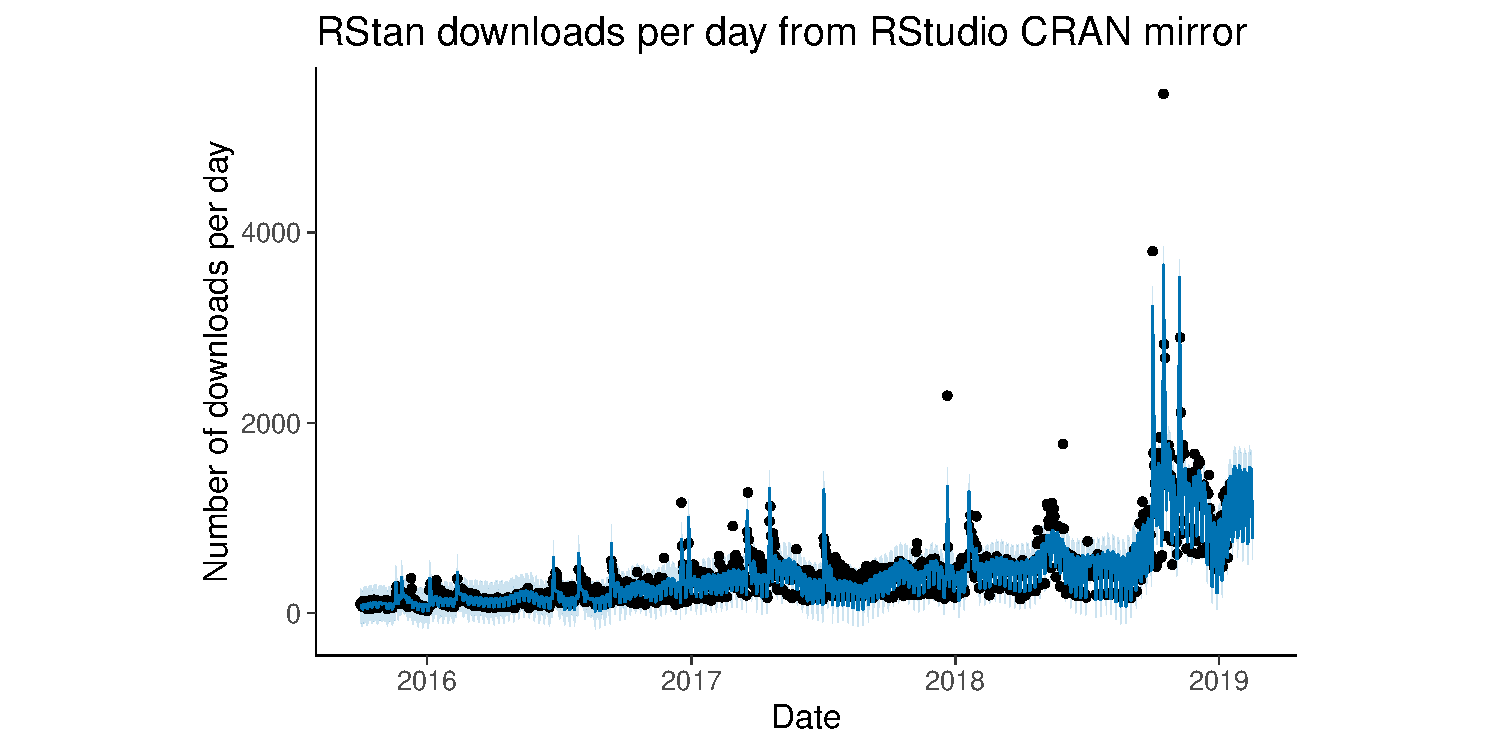
\includegraphics[width=16cm]{rstan_downloads_forecast.pdf}}
    \only<2>{\hspace*{-2.5cm}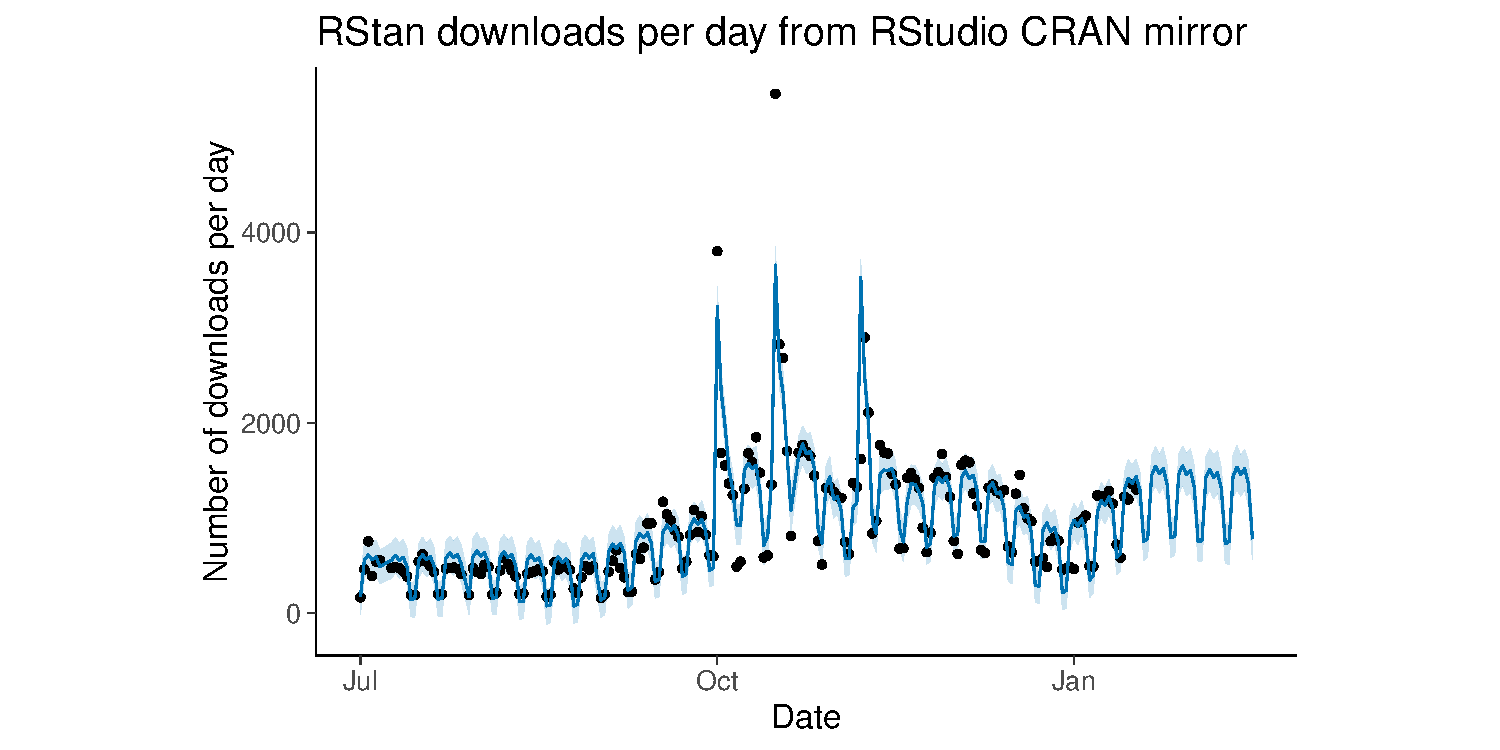
\includegraphics[width=16cm]{rstan_downloads_forecast_zoomed.pdf}}
    \only<3>{\hspace*{-.5cm}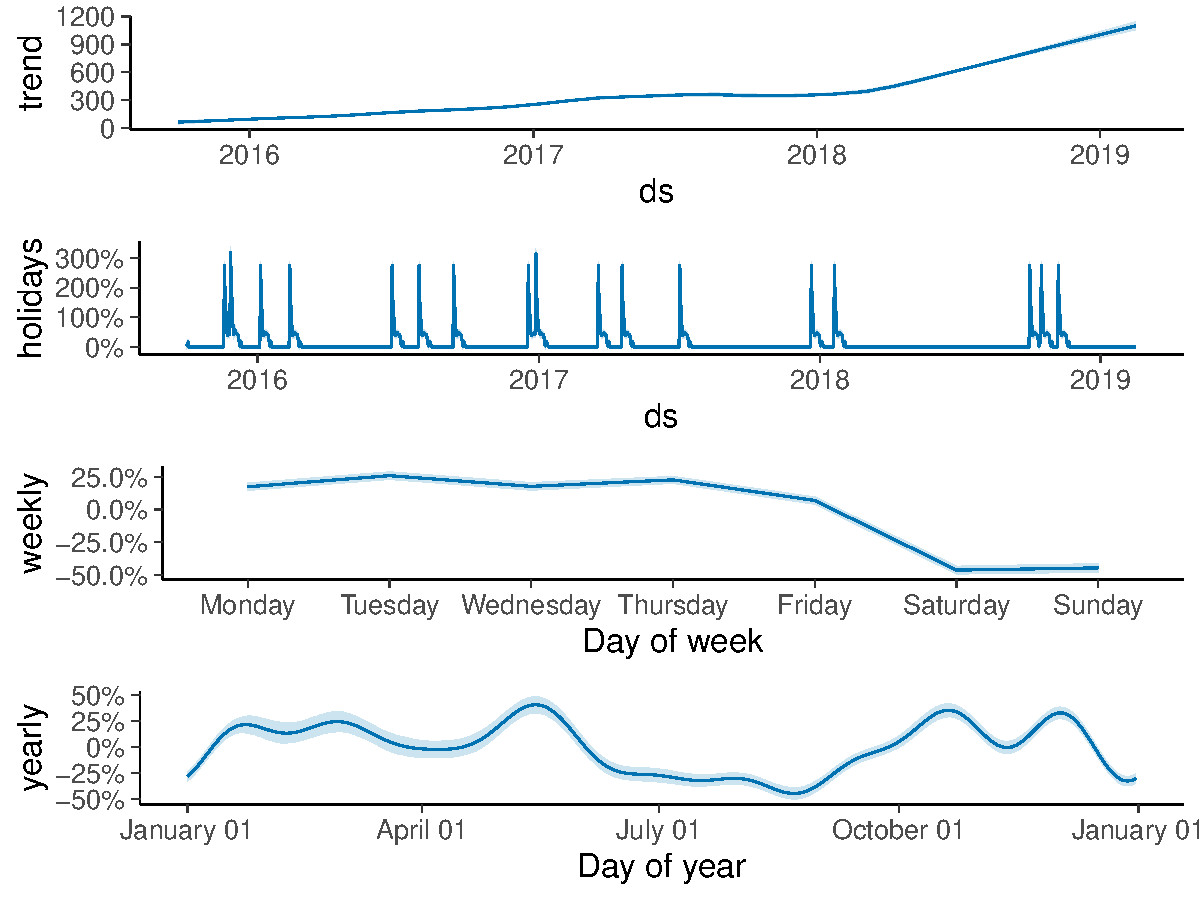
\includegraphics[width=11.25cm]{rstan_downloads_components.pdf}}
  
\end{frame}

%skip rest in video

\begin{frame}
  \frametitle{Sufficient statistics*}

  \begin{itemize}
  \item The quantity $t(y)$ is said to be a {\em sufficient statistic}
    for $\theta$, because the likelihood for $\theta$ depends on the
    data $y$ only through the value of $t(y)$.
  \end{itemize}

\end{frame}

%%% demos

\begin{frame}
  \frametitle{Posterior visualization and inference demos}

  \begin{itemize}
  \item demo2\_3: Simulate samples from Beta(438,544), and draw
    a histogram of $\theta$ with quantiles.
  \end{itemize}
  \vspace{-\baselineskip}
  \begin{center}
  \includegraphics[width=11cm]{figs/demo2_3.pdf}
\end{center}
\end{frame}

\begin{frame}
  \frametitle{Posterior visualization and inference demos}

  \begin{itemize}
  \item demo2\_4: Compute posterior distribution in a grid.
  \end{itemize}
  \includegraphics[width=11cm]{figs/demo2_4a.pdf}
\end{frame}

\begin{frame}
  \frametitle{Posterior visualization and inference demos}

  \begin{itemize}
  \item demo2\_4: Sample using the inverse-cdf method.
  \end{itemize}
  \includegraphics[width=11cm]{figs/demo2_4b.pdf}
\end{frame}

\begin{frame}
  \frametitle{Algae}
  \framesubtitle{Exercise}

Algae status is monitored in 274 sites at Finnish lakes and rivers. 
The observations for the 2008 algae status at each site are presented
in file \emph{algae.mat} ('0': no algae, '1': algae present). 
% In year 2008 blue-green algae was observed at 44 sites. 
Let $\pi$ be the probability of a monitoring site having detectable
blue-green algae levels. 

\begin{itemize}
\item Use a binomial model for observations and a \emph{beta}(2,10) prior.
\item What can you say about the value of the unknown $\pi$?
\item Experiment how the result changes if you change the prior.
\end{itemize}

\end{frame}

%%%normal

\begin{frame}
  \frametitle{Normal / Gaussian}

  \begin{itemize}
  \item Observations $y$ real valued
  \item Mean $\theta$ and variance $\sigma^2$ (or deviation $\sigma$)\\
    (first assume $\sigma^2$ known)
  \end{itemize}
  \vskip -2mm
  \begin{align*}
    p(y|\theta)&=\frac{1}{\sqrt{2\pi}\sigma}\exp\left(-\frac{1}{2\sigma^2}(y-\theta)^2\right)\\
    y & \sim \N(\theta,\sigma^2)
  \end{align*}

  \begin{center}
      \includegraphics[clip]{kuva2b_1}
  \end{center}
\end{frame}

\begin{frame}

  \frametitle{Reasons to use Normal distribution}

  \begin{itemize}
  \item Normal distribution often justified based on central limit theorem
  \item More often used due to the computational convenience or tradition
  \end{itemize}

\end{frame}

%%skip in video

\begin{frame}

  \frametitle{Central limit theorem*}

  \begin{itemize}
  \item De Moivre, Laplace, Gauss, Chebysev, Liapounov, Markov, et al.
  \item Given certain conditions sum (and mean) of random variables
    approach Gaussian distribution as d $n \rightarrow \infty$
  \item Problems
    \begin{itemize}
    \item does not hold for all distributions, e.g., Cauchy
    \item may require large $n$,\\ e.g.
      Binomial, when $\theta$ close to $0$ or $1$
    \item does not hold if one the variables has much larger scale
    \end{itemize}
  \end{itemize}

\end{frame}

% \begin{frame}
%  \frametitle{Normal distribution - conjugate prior for $\theta$}

%  \begin{itemize}
%  \item Assume $\sigma^2$ known
%    \begin{align*}
%      &\text{Likelihood} & p(y|\theta) & \propto
%      \exp\left(-\frac{1}{2\sigma^2}(y-\theta)^2\right)\\ \\
%      &\text{Prior} & p(\theta) & \propto \exp\left(-\frac{1}{2\tau_0^2}(\theta-\mu_0)^2\right)
%    \end{align*}
% \end{itemize}
% \end{frame}

\begin{frame}
  \frametitle{Normal distribution - conjugate prior for $\theta$}

  \begin{itemize}
  \item Assume $\sigma^2$ known
    \begin{align*}
      &\text{Likelihood} & p(y|\theta) & \propto
      \exp\left(-\frac{1}{2\sigma^2}(y-\theta)^2\right)\\ \\
      &\text{Prior} & p(\theta) & \propto
      \exp\left(-\frac{1}{2\tau_0^2}(\theta-\mu_0)^2\right)\\ \\
      & & \uncover<2->{\exp(a)\exp(b)} & \uncover<2->{= \exp(a+b)} \\ \\
      &\uncover<3->{ \text{Posterior}}&
      \uncover<3->{p(\theta|y)& \propto \exp\left(-\frac{1}{2}\left[ \frac{(y-\theta)^2}{\sigma^2}+\frac{(\theta-\mu_0)^2}{\tau_0^2} \right]\right)}
    \end{align*}
  \end{itemize}

\end{frame}

% \note{  exp(a)*exp(b)=exp(a+b)}

 \begin{frame}
  \frametitle{Normal distribution - conjugate prior for $\theta$}

  \begin{itemize}
  \item Posterior (see ex 2.14a)
    \vskip -5mm
    \begin{align*}
      & &
      p(\theta|y)&\propto \exp\left(-\frac{1}{2}\left[
          \frac{(y-\theta)^2}{\sigma^2}+\frac{(\theta-\mu_0)^2}{\tau_0^2} \right]\right) \\ 
      & & & \propto \exp \left(-\frac{1}{2\tau_1^2}(\theta-\mu_1)^2
      \right)
    \end{align*}
    \begin{equation*}
      \theta|y \sim \N(\mu_1,\tau_1^2), \quad
      \text{where} \quad
      \mu_1=\frac{\frac{1}{\tau_0^2}\mu_0+\frac{1}{\sigma^2}y}{\frac{1}{\tau_0^2}+\frac{1}{\sigma^2}} \quad  \text{and}  \quad \frac{1}{\tau_1^2} = \frac{1}{\tau_0^2}+\frac{1}{\sigma^2}
    \end{equation*}
    \vskip -2mm
    \pause
    \item 1/variance = precision
    \item Posterior precision = prior precision + data precision
    \item Posterior mean is precision weighted mean
  \end{itemize}


\end{frame}

\begin{frame}
  \frametitle{Normal distribution - example}

  \only<1>{\includegraphics[width=11cm]{pguess.pdf}}
  \only<2>{\includegraphics[width=11cm]{pguessprior.pdf}}
  \only<3>{\includegraphics[width=11cm]{ppost.pdf}}
  
\end{frame}

\begin{frame}
  \frametitle{Normal distribution - conjugate prior for $\theta$}

  \begin{itemize}
  \item Several observations -- use chain rule
  \end{itemize}

\end{frame}

\begin{frame}

  \frametitle{Normal distribution - conjugate prior for $\theta$}

  \begin{itemize}
  \item Several observations $y=(y_1,\ldots,y_n)$
    \begin{align*}
      p(\theta|y) = \N(\theta|\mu_n,\tau_n^2)
    \end{align*}
    \vskip -6mm
    \begin{align*}
      \text{where} \quad
      \mu_n=\frac{\frac{1}{\tau_0^2}\mu_0+\frac{n}{\sigma^2}\bar{y}}{\frac{1}{\tau_0^2}+\frac{n}{\sigma^2}} \quad
      \text{ja} \quad \frac{1}{\tau_n^2} = \frac{1}{\tau_0^2}+\frac{n}{\sigma^2}
    \end{align*}
  \item If $\tau_0^2=\sigma^2$, prior corresponds to one virtual observation with value $\mu_0$
    \pause
    \item If $\tau_0\rightarrow\infty$ when $n$ fixed\\
      or if $n\rightarrow\infty$ when $\tau_0$ fixed
      \begin{equation*}
        p(\theta|y) \approx \N(\theta|\bar{y},\sigma^2/n)
      \end{equation*}
  \end{itemize}

\end{frame}

\begin{frame}
  \frametitle{Normal distribution - conjugate prior for $\theta$}

  \begin{itemize}
  \item Posterior predictive distribution
    \begin{align*}
      p(\tilde{y}|y)&=\int p(\tilde{y}|\theta)p(\theta|y) d\theta \\
      p(\tilde{y}|y)& \propto\int
      \exp\left(-\frac{1}{2\sigma^2}(\tilde{y}-\theta)^2\right)\exp\left(-\frac{1}{2\tau_1^2}(\theta-\mu_1)^2\right) d\theta \\
      ~&~\\ 
      \tilde{y}|y &\sim \N(\mu_1,\sigma^2+\tau_1^2)
    \end{align*}
  \item Predictive variance = observation model variance $\sigma^2$ + \\
     posterior variance $\tau_1^2$

  \end{itemize}

\end{frame}

 % \begin{frame}
 %   \frametitle{Some other one parameter models}

 %   \begin{itemize}
 %   \item Poisson
 %   \item Exponential
 %   \item Cauchy
 %   \end{itemize}
   
 % \end{frame}


\end{document}

%%% Local Variables: 
%%% TeX-PDF-mode: t
%%% TeX-master: t
%%% End: 
